%%%%%%%%%%%%%%%%%%%%%%%%%%%%%%%%%%%%%%%%%
% Lachaise Assignment
% LaTeX Template
% Version 1.0 (26/6/2018)
%
% This template originates from:
% http://www.LaTeXTemplates.com
%
% Authors:
% Marion Lachaise & François Févotte
% Vel (vel@LaTeXTemplates.com)
%
% License:
% CC BY-NC-SA 3.0 (http://creativecommons.org/licenses/by-nc-sa/3.0/)
% 
%%%%%%%%%%%%%%%%%%%%%%%%%%%%%%%%%%%%%%%%%

%----------------------------------------------------------------------------------------
%	PACKAGES AND OTHER DOCUMENT CONFIGURATIONS
%----------------------------------------------------------------------------------------

\documentclass{article}
\usepackage{graphicx}
\graphicspath{{images/}}
\usepackage{float} 
\usepackage{tikz, tikz-cd}
\usepackage{mathtools}
\usepackage{pgfplots}
\usetikzlibrary{spy}
\pgfplotsset{width=10cm,compat=1.18}
\input{structure.tex} % Include the file specifying the document structure and custom commands
\renewcommand{\figurename}{Figura}
\usepackage{tcolorbox}
\usepackage{lipsum}
\tcbuselibrary{listings,theorems,skins,vignette,raster,breakable,magazine,poster,fitting,hooks}
%----------------------------------------------------------------------------------------
%	ASSIGNMENT INFORMATION
%----------------------------------------------------------------------------------------

\title{AMPLIFICADOR LOGARÍTMICO} % Title of the assignment

\author{Rodrigo Castillejos} % Author name and email address

\date{castillejosm.rodrigo@gmail.com} % University, school and/or department name(s) and a date

%----------------------------------------------------------------------------------------

\begin{document}

\maketitle % Print the title

%----------------------------------------------------------------------------------------
%	INTRODUCTION
%----------------------------------------------------------------------------------------

\section*{Amplificador logarítmico} % Unnumbered section
La conversión de una señal a su valor logarítmico equivalente involucra una operación no lineal. Muchos de los conceptos de los circuitos lineales son irrelevantes en el uso de amplificadores logarítmicos. Por ejemplo, la ganancia incremental de un amplificador logarítmico ideal tiende a menos infinito conforme la entrada tiende a cero.\\

\noindent Si consideramos la ecuación $y=log(x)$ encontramos que cada vez que $X$ sea multiplicado or una constante $A$, $Y$ se incrementa por otra constante $A_1$. Así, si $log(K) = K_1$, entonces $log(AK) = K_1 + A_1$, $log(A^{2}K) = 2A_1 + K_1$, y $log(K/A) = K_1 - A_1$. Esto proporciona una gráfica como se muestra en la figura \ref{fig:figura1}.  
\begin{figure}[H]
	\centering
	
\includegraphics[scale=0.5]{figura1}
	\caption{Gráfica de $y = log(x)$}
	\label{fig:figura1}
\end{figure}

\noindent El circuito de amplificador logarítmico más fundamental se muestra en la figura \ref{fig:log_amp}. La corriente de colector $i_C$ es igual a la forma de un diodo ideal
\begin{equation}
	i_C = I_S\left[ \exp\left({ \frac{v_{BE}}{V_T} }\right) - 1 \right]
\end{equation}
\noindent El parámetro $I_S$ es la \textbf{corriente de saturación del transistor}. Esto es, la corriente de saturación del transistor bipolar. $I_S$ es proporcional al área de sección transversal de la región de base activa del transistor, y puede tener un amplio rango de valores:
\begin{align}
	10^{-18} A \leq I_S \leq 10^{-9} A\nonumber 
\end{align}
\noindent En la ecuación (1), $V_T$ es el voltaje térmico y está dado por $V_T = kT/q \simeq 0.025V$ a temperatura ambiente. 

\begin{figure}[H]
	\centering
	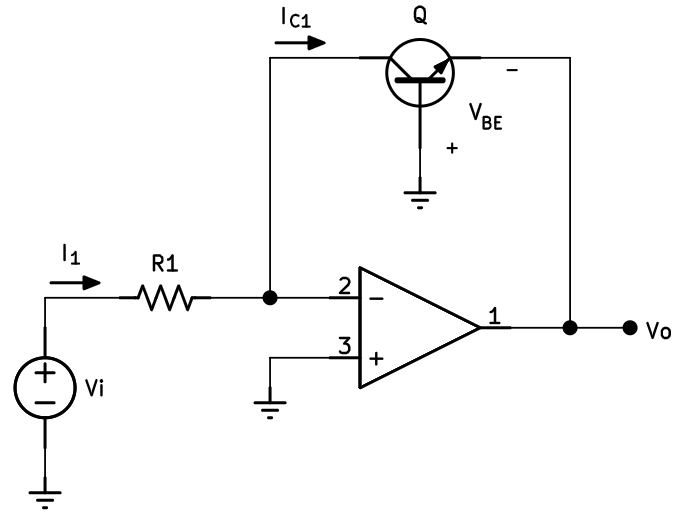
\includegraphics[scale=0.7]{figura2}
	\caption{Amplificador logarítmico fundamental.}
	\label{fig:figura2}
\end{figure}

\noindent Debido a la muy baja corriente de saturación es posible eliminar el término constante, por lo tanto
\begin{align}
	i_C = I_S \, e^{ \frac{v_{BE}}{V_T} }
\end{align}

\noindent Si aplicamos la LCK sobre la entrada del amplificador de la figura \ref{fig:log_amp} obtenemos
\begin{align}
	i_1 = i_{C1}
\end{align}

\noindent O bien
\begin{align}
	\frac{V_i}{R_1} = I_S \, e^{ \frac{V_{BE}}{V_T} }
\end{align}
\noindent Al aplicar la LTK sobre el lazo que comprende a la unión base-emisor y la salida del amplificador obtenemos:
\begin{align}
	v_O + v_{BE} = 0\nonumber
\end{align}
\noindent Es decir
\begin{align}
	v_O &= -v_{BE}
\end{align}

\noindent De esta manera, despejamos el voltaje $v_{BE}$ de la ecuación (4)	
\begin{align}
	\frac{V_i}{R_1I_S} = e^{ \frac{v_{BE}}{V_T} }\nonumber\\
	\ln \left( \frac{V_i}{R_1I_S} \right) = \frac{v_{BE}}{V_T}\nonumber
\end{align}
\noindent Por lo tanto
\begin{align}
	v_{BE} = V_T \ln \left( \frac{V_i}{R_1I_S} \right)
\end{align}

\noindent Es fácil visualizar voltaje de salida para el amplificador logarítmico básico usando la ecuación (5) 	

\begin{tcolorbox}[colback=red!5!white,colframe=red!75!black,arc=0mm,boxrule=0mm,width=(\linewidth+0.5cm),extrude right by=-1.5cm]
	\begin{equation}
		v_O = - V_T \ln \left( \frac{V_i}{R_1I_S} \right) = - V_T \ln \left( \frac{V_i}{V_{ref}} \right)
	\end{equation}
\end{tcolorbox}

\noindent Donde 
\begin{align}
	V_{ref} = R_1I_S\nonumber
\end{align}
Este circuito, sin embargo, tiene un problema. La corriente de saturación $I_S$ varía de transistor a transistor y con la temperatura, por lo tanto no es posible obtener un voltaje de referencia estable. Esta dependencia a $I_S$ se puede eliminar utilizando el circuito propuesto de la figura \ref{fig:log_amp1}.

\begin{figure}[H]
	\centering
	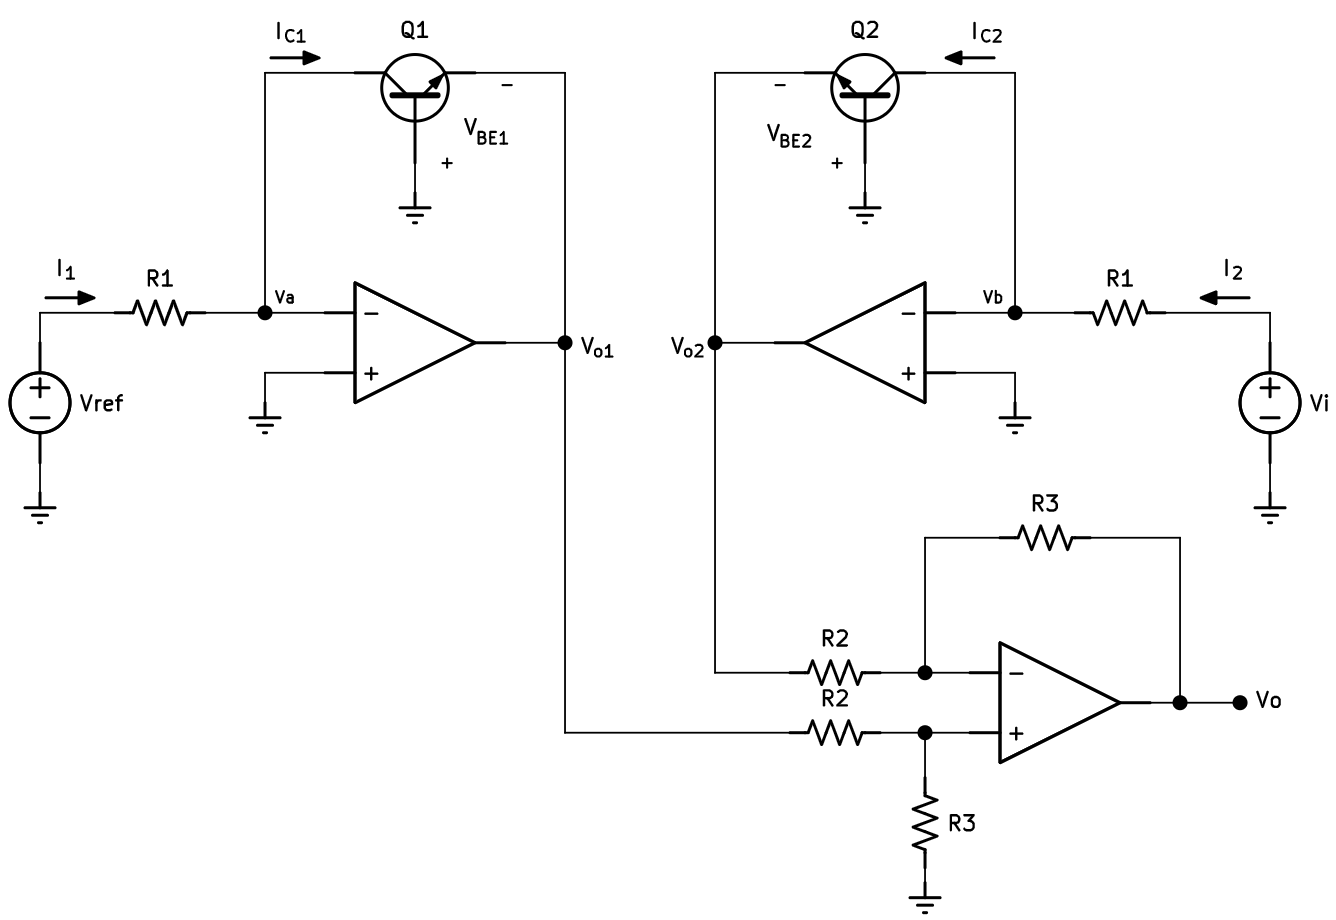
\includegraphics[scale=0.6]{log_amp1}
	\caption{Amplificador logarítmico mejorado}
	\label{fig:log_amp1}
\end{figure}

\noindent Con base en el análisis efectuado anteriormente es posible determinar rápidamente los voltajes $V_{o1}$ y $V_{o2}$, es decir
\begin{align}
	V_{o1} = - V_T \ln \left( \frac{V_{ref}}{R_1I_S} \right)\\
	V_{o2} = - V_T \ln \left( \frac{V_i}{R_1I_S} \right)
\end{align}
\noindent Las salidas de los amplificadores logarítmicos están conectados a un amplificador diferencial, en cuanto a este amplificador sabemos que la salida $Vo$ es:

\begin{align}
	V_o = \frac{R_3}{R_2}(V_{o1} - V_{o2})
\end{align}

\noindent La sustitución de las ecuaciones (8) y (9) en (10) produce
\begin{align}
	V_o &= \frac{R_3}{R_2} \left[ - V_T \ln \left( \frac{V_{ref}}{R_1I_S} \right) + V_T \ln \left( \frac{V_i}{R_1I_S} \right) \right]\nonumber\\
	&= V_T \frac{R_3}{R_2} \left[ \ln \left( \frac{V_i}{R_1I_S} \right) - V_T \ln \left( \frac{V_{ref}}{R_1I_S} \right)  \right]\nonumber
\end{align}
\begin{align}
	V_o = V_T \frac{R_3}{R_2} \ln \left( \frac{V_i}{V_{ref}} \right)
\end{align}

\noindent Realizaremos un cambio de base con el fin de expresar el voltaje de salida en términos de logaritmo en base 10. Recordemos que

\begin{tcolorbox}[colback=red!5!white,colframe=red!75!black,arc=0mm,boxrule=0mm,width=(\linewidth+0.5cm),extrude right by=-1.5cm]
	\begin{equation}
		\log_{b}N = \frac{\log_{a}N}{\log_{a}b}
	\end{equation}
\end{tcolorbox}

\noindent Donde 
\begin{subequations}
	\begin{align}
		b &= e\\
		N &= \frac{V_i}{V_{ref}}\\
		a &= 10
	\end{align}
\end{subequations}

\noindent Así
\begin{align}
	\log_{e}\left( \frac{V_i}{V_{ref}} \right) = \frac{ \log_{10}\left( \frac{V_i}{V_{ref}} \right) }{ \log_{10}e } = \frac{ \log_{10}\left( \frac{V_i}{V_{ref}} \right) }{0.4343}
\end{align}
\noindent Para el amplificador logarítmico de la figura 2, asumiendo que $Q_1$ y $Q_2$ son transistores emparejados. El objetivo es encontrar los valores de $R_2$ Y $R_3$ de tal manera que el voltaje de salida está dado por
\begin{align}
	V_o = 1.0\, \log _{10}\left( \frac{V_i}{V_{ref}} \right)\nonumber
\end{align}

\noindent Sustituimos la ecuación (14) en (11)
\begin{align}
	V_o = 2.3V_T \frac{R_3}{R_2} \log_{10} \left( \frac{V_i}{V_{ref}} \right)
\end{align}

\noindent \textbf{Análisis de sensibilidad}\\
En el diseño de cualquier circuito electrónico, la tolerancia en los valores de los componentes, así como los voltajes y corrientes de referencia pueden causar una desviación sobre la salida deseada del sistema. Sin embargo, la desviación de la salida del sistema debido a la variación de cada una de sus entradas es diferente. La salida puede llegar a ser más sensible a ciertas entradas que otras.\\

\noindent El análisis de sensibilidad es el estudio de cómo un cierto sistema reacciona reacciona a sus entradas. Es una técnica de análisis para variables que cambian sistemáticamente dentro de un modelo y determinar los efectos de tales cambios en su salida.
Debido a la tolerancia en los valores de los componentes, como resistores, capacitores, inductores, e incluso voltaje y corrientes de referencia, el análisis de sensibilidad es una poderosa técnica usada en el diseño de circuitos. Ayuda a determinar el efecto de cada tolerancia de entrada dentro del sistema y su efecto sobre el rendimiento general del modelo. la función de sensibilidad clásica se define como 

\begin{tcolorbox}[colback=red!5!white,colframe=red!75!black,arc=0mm,boxrule=0mm,width=(\linewidth+0.5cm),extrude right by=-1.5cm]
	\begin{equation}
		\scalebox{1.5}{S}_x^{y} = \frac{\partial y}{\partial x} \frac{x}{y}
	\end{equation}
\end{tcolorbox}

\noindent $x$ representa el valor de los componentes tales como resistores , capacitores, inductores, referencias de voltaje, etc., $y$ representa el parámetro de salida de interés como la frecuencia, fase, voltaje de salida o corriente de salida.. el resultado de la sensibilidad determina el cambio por unidad en $y$ debido a un cambio por unidad en $x$.

\noindent Para determinar qué tanto afecta al sistema cualquier cambio en la temperatura podemos escribir la siguiente ecuación

\begin{align}
	\scalebox{1.8}{S}_{V_T}^{V_o} = \frac{\partial V_o}{\partial V_T} \frac{V_T}{V_o}
\end{align}

\noindent Donde
\begin{align}
	\frac{\partial V_o}{\partial V_T} = \frac{\partial}{\partial V_T}\left( 2.3V_T \frac{R_3}{R_2} \log_{10} \left(\frac{V_i}{V_{ref}}\right) \right) = 2.3V_T \frac{R_3}{R_2}\log_{10}\left( \frac{V_i}{V_{ref}} \right)
\end{align}

\noindent Así
\begin{align}
	\scalebox{1.8}{S}_{V_T}^{V_o} = 2.3V_T \frac{R_3}{R_2}\log_{10}\left( \frac{V_i}{V_{ref}} \right) \frac{V_T}{ 2.3V_T \frac{R_3}{R_2} \log_{10} \left( \frac{V_i}{V_{ref}} \right) } = V_T
\end{align}

Recordemos que $V_T$, (el voltaje térmico) está dado por
\begin{align}
	V_T = \frac{kT}{q}
\end{align}

\noindent Donde:\\
$k$ = la contante de Boltzmann, $ = 8.62 \times 10^{-5} \frac{eV}{K}$\\
$T$ =  la temperatura absoluta en kelvins $=273.15 + C^{\circ} $\\
$q$ = la magnitud de la carga eléctrica $= 1.60 \times 10^{-19}$ coulomb \\

\noindent A una temperatura ambiente de $25^{\circ}C$ el voltaje térmico será de
\begin{align}
	V_T = \frac{kT}{q} = \frac{(8.62 \times 10^{-4} eV/K)(273.15 + 25)K}{1.602 \times 10^{-19} C} = 160.6283 \times 10^{15} \frac{eV}{C}
\end{align}

\noindent Sin embargo, $1C = 6.24\times 10^{18}e$, así
\begin{align}
	V_T = \left( 160.6283 \times 10^{15} \frac{eV}{C} \right) \left( \frac{1C}{6.24 \times 10^{18}\,e} \right) \simeq 0.0258 \, V = 25.8 \,mV\nonumber
\end{align}

\noindent Para hacer que la ecuación (15) sea igual a
\begin{align}
	V_o = 1.0 \log_{10} \left( \frac{V_i}{V_{ref}} \right)\nonumber
\end{align}

\noindent Tenemos que hacer que el término constante $2.3V_T \frac{R_3}{R_2}$ sea igual a $1$, por lo tanto:
\begin{align}
	2.3V_T \frac{R_3}{R_2} = 1\nonumber\\
	\frac{R_3}{R_2} = 16.852\nonumber\\
	R_3 = 16.852R_2
\end{align}

\end{document}
